\documentclass[a4paper,12pt]{article}
\usepackage[paper=a4paper,left=35mm,right=25mm,top=25mm,bottom=20mm]{geometry}
\usepackage[ngerman]{babel}
\usepackage[utf8]{inputenc}
\usepackage{amsmath}
\usepackage{amssymb}
\usepackage{tikz}
\usepackage{pgfplots}
\usepackage{enumitem}
\usepackage{cite}
\usepackage[square,sort,comma,numbers]{natbib}
\usepackage{graphicx}
\usepackage{float}

\linespread{1.5}

\addto\captionsngerman{
  \renewcommand{\contentsname}
    {INHALTSVERZEICHNIS}
}


\begin{document}
\parindent0cm
\setlength{\abovedisplayskip}{-1cm}
\setlength{\belowdisplayskip}{0.75cm}

%===================================================================================
%---------------------------- TITELSEITE -------------------------------------------
%===================================================================================

\thispagestyle{empty}

\begin{center}

\begin{large} 
GYMNASIUM OTTOBRUNN	\\
\vspace{1cm}
Oberstufenjahrgang 2017/19\\
\vspace{1cm}
Seminarfach Softwareentwicklung\\
\vspace{2cm}
Seminararbeit\\
\end{large}


\vspace{1cm}


{\Huge\bfseries 
36. Bundeswettbewerb Informatik\par
Runde 2\par
Aufgabe 1 und 3\par 
}


\vspace{2cm}


\begin{large}
\begin{tabular}{rl}
Verfasser:& Jonas Fritsch \\
Seminarleiter: & StD Peter Brichzin \\
Bewertung:  & ......... Punkte  \\
Unterschrift des Seminarleiters: & ...........................................  \\
\end{tabular} 
\end{large}

\end{center}

%===================================================================================
%---------------------------- INHALTSVERZEICHNIS -----------------------------------
%===================================================================================				

\newpage

\thispagestyle{empty}
\tableofcontents	


\setcounter{page}{2}

%===================================================================================
%-------------------------------- EINLEITUNG ---------------------------------------
%===================================================================================

\newpage
\section{EINLEITUNG}



Lorem ipsum dolor sit amet, consectetur adipiscing elit. Sed tempus consectetur lorem, imperdiet dignissim est auctor a. Vivamus convallis, leo et iaculis egestas, nunc massa porttitor tellus, id faucibus urna justo eget massa. Praesent quis feugiat odio. Nullam quis mattis enim. Fusce volutpat odio in enim sodales venenatis. Mauris consequat.

%===================================================================================
%-------------------------------- AUFGABE 1 ----------------------------------------
%===================================================================================

\newpage
\section{AUFGABE 1 - "Die Kunst der Fuge"}



\subsection{Aufgabenstellung}
Ilona besitzt einen riesigen Haufen Holzklötzchen: Diese haben alle dieselbe Höhe und Tiefe,
aber verschiedene Längen. \\
Ilona möchte eine Mauer bauen. Jede Reihe der Mauer soll aus $n$ Klötzchen bestehen, die die
Längen 1 bis $n$ haben und lückenlos aneinander liegen. Die Stellen zwischen den Klötzchen heißen
Fugen. Ilona möchte, dass in der fertigen Mauer niemals zwei Fugen übereinander liegen,
selbst wenn sich mehrere Reihen dazwischen befinden. Außerdem soll ihre Mauer möglichst
hoch sein. \\
Für $n = 4$ gelingt es ihr recht schnell, eine Mauer mit drei Reihen zu bauen:
\begin{figure}[H]
    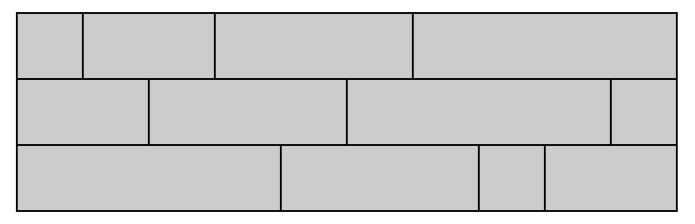
\includegraphics[width=0.7\linewidth]{Bilder/Aufgabe1/Aufgabenstellung_BeispielMauer.png}
\end{figure}
\begin{large}
    \textbf{Aufgabe} \\
\end{large}
Hilf Ilona, indem du ein Programm schreibst, das nach Eingabe von $n$ eine nach ihren Vorgaben
konstruierte, möglichst hohe Mauer ausgibt. Für $n = 10$ sollte dein Programm eine Mauer der
Höhe 6 ausgeben können. Wie hoch werden die Mauern deines Programms für größere $n$?

\subsection{Auslegung der Aufgabe}
Die grundlegende Aufgabe ist, eine Mauer mit möglichst vielen Reihen, die aus verschieden länglichen Klötzchen bestehen, zu bauen.

Die Längen der Klötzchen in einer Reihe sind durch eine Variable $n$ definiert.
Die Variable $n$ ($n \in \mathbb{N}$\textbackslash$\{0\}$) definiert dabei die Längen und auch die Gesamtanzahl der Klötzchen pro Reihe.
Gesamtanzahl heißt, dass bei zum Beispiel $n = 5$ jede Reihe aus 5 einzelnen Klötzchen besteht. 
Jede Reihe setzt sich dann aus einem 1er, einem 2er, einem 3er, einem 4er und einem 5er Klotz zusammen.
\\[0.4cm]
Der Trick bei der Aufgabe ist nun, dass niemals zwei Fugen \textbf{übereinanderliegen dürfen}.
Eine Fuge ist die Lücke zwischen zwei Klötzchen (siehe Abbildung 1).
\begin{figure}[H]
    \centering
    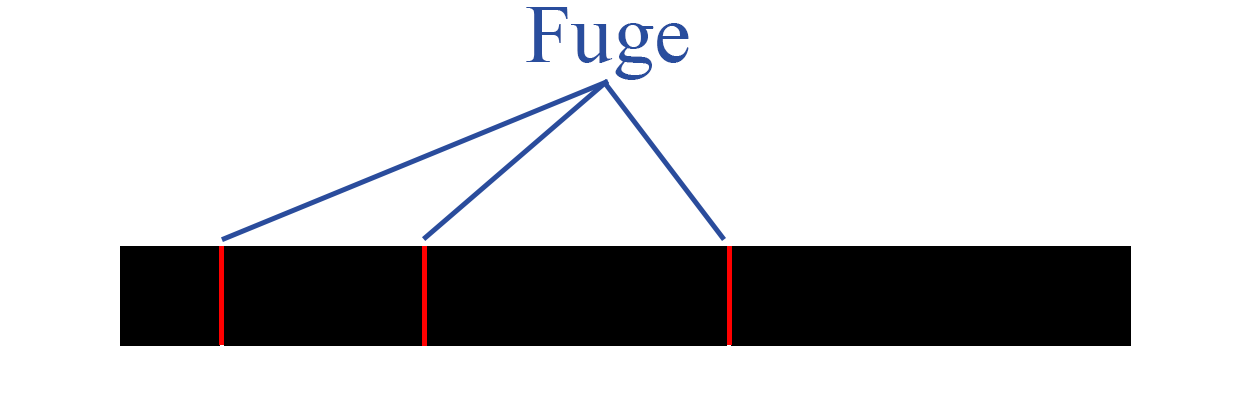
\includegraphics[width=0.8\linewidth]{Bilder/Aufgabe1/Definition_Fuge.png}
    \caption{Darstellung der 3 Fugen einer Reihe mit 4 Klötzchen}
\end{figure}

Als Hilfestellung wurde außerdem erwähnt, dass eine Mauer für $n = 10$ eine maximale Höhe von $6$ hat.

\subsection{Lösungsidee}
\subsubsection{Verstehen des Problems}
Um die Problemstellung der Aufgabe genauer zu verstehen, bietet es sich erstmal an, Mauern für kleinere $n$ auf Papier zu zeichnen.
Beginnt man mit $n = 1$, fällt auf, dass ganz gleich wie viele Reihen übereinanderliegen, es nie zu einer Fugenüberlappung kommen kann, da eine Reihe mit einem einzelnen Klötzchen keine Fuge besitzt.
Für $n = 1$ kann also theoretisch eine \textbf{unendlich} hohe Mauer gebaut werden.
\\[0.4cm]
Für $n = 2$ ist es auch noch recht einfach, eine Mauer zu bauen. Denn es gibt pro Reihe nur 2 mögliche Reihenfolgen von Klötzchen. Entweder kommt zuerst der 1er oder der 2er Klotz. 
Eine der zwei möglichen Lösungen ist in Abbildung 2 zu sehen. Es gibt keine Möglichkeit, noch ein Klötzchen mehr zu platzieren, ohne eine Fuge doppelt zu besetzen.
\begin{figure}[H]
    \centering
    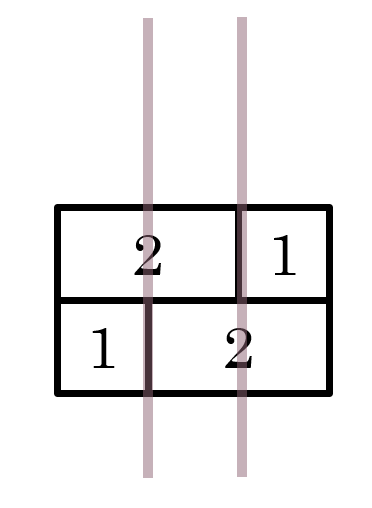
\includegraphics[width=0.3\linewidth]{Bilder/Aufgabe1/Loesung_N2.png}
    \caption{Eine der zwei möglichen Lösungen für $n = 2$. Die roten Striche zeigen an, dass die jeweilige Fuge bereits besetzt ist.}
\end{figure}

Auch für $n = 3$ gibt es eine Mauer mit einer maximalen Höhe von 2 (siehe Abbildung 3). Hier wird es jedoch schon komplexer, da es nun für eine Reihe nicht mehr $2! = 2\times1 = 2$, sondern $3! = 3\times2\times1 = 6$ mögliche Klötzchen-Reihenfolgen gibt.
Außerdem tritt bei $N = 3$ das erste Mal auf, dass eine \textbf{mögliche Fugenstelle nicht besetzt wird.}
\begin{figure}[H]
    \centering
    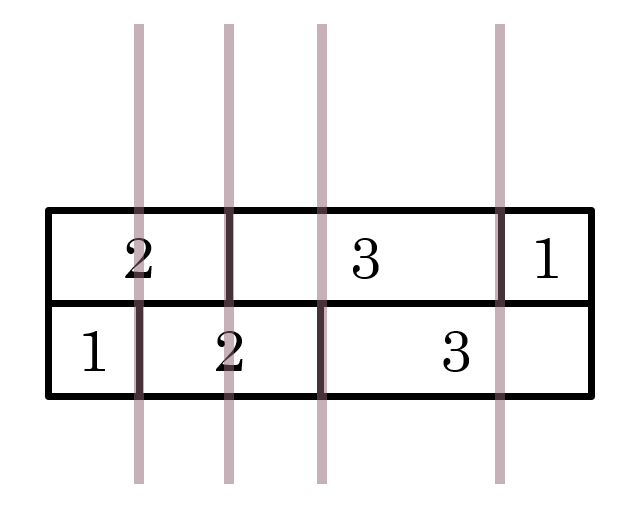
\includegraphics[width=0.5\linewidth]{Bilder/Aufgabe1/Loesung_N3.png}
    \caption{Eine mögliche Lösung für $n = 3$. Zu beachten ist, dass in der Mauer eine \textbf{mögliche} Fugenstelle, dort wo es eine größere Lücke zwischen den zwei letzten besetzten Fugenstellen gibt, \textbf{unbesetzt bleibt.}}
\end{figure}

Geht man noch weiter und bildet eine Mauer für $n = 4$ ($4! = 24$ mögliche Klötzchen Anordnungen pro Reihe), so kann man erstmals eine Mauer der Höhe 3 bilden (siehe Abbildung 4). Hier ist auch wieder jede einzelne Fugenstelle besetzt.
\begin{figure}[H]
    \centering
    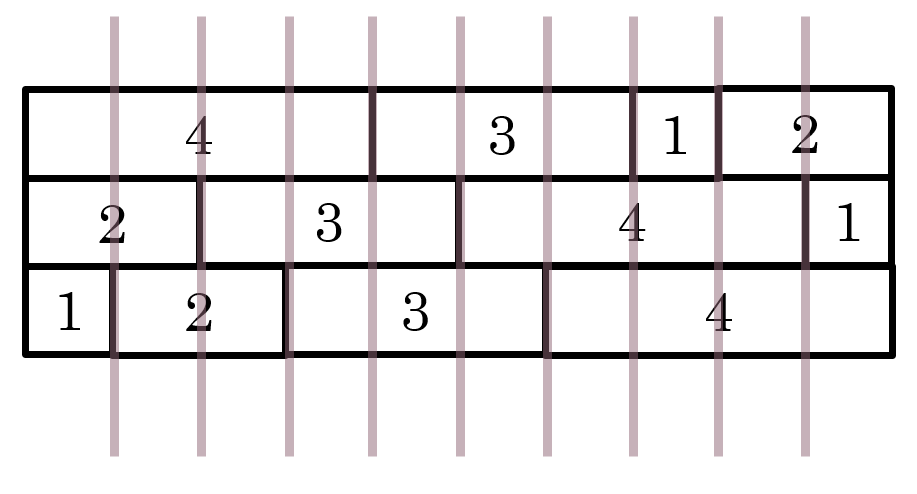
\includegraphics[width=0.7\linewidth]{Bilder/Aufgabe1/Loesung_N4.png}
    \caption{Eine mögliche Lösung für $n = 4$}
\end{figure}

Die Komplexität der Aufgabe steigt mit höheren $n$ stark an. Während man bei $n = 2 2!$ Möglichkeiten pro Reihe und 2 Reihen hatte ($2!\times2 = 4$ unterschiedliche Lösungen), gibt es bei $n = 4$ bereits $4!\times3 = 72$ verschiedene Lösungen.
Allgemein gibt es also für eine Mauer $n!\times h$ Lösungen, wobei $h$ die Anzahl der übereinanderliegenden Reihen ist.
\\[0.4cm]
Es ist logisch, dass zwischen der Anzahl der maximal möglichen Reihen $h$ und der Anzahl der Klötzchen pro Reihe $n$ eine Abhängigkeit existiert.
\\[0.4cm]
Allgemein kann man sagen, dass die \textbf{maximale Mauerhöhe} dann erreicht ist, wenn \textbf{nicht} mehr \textbf{genug Fugenstellen in der Mauer frei sind}, um eine \textbf{weitere Reihe zu bilden}.

Somit lässt sich die Formel
\begin{center}
\begin{Large}
\[h = \frac{f_{Mauer}}{f_{Reihe}}\]
\end{Large}
\end{center}
ableiten, wobei $f_{Mauer}$ die maximale Anzahl an Fugen in der Mauer und $f_{Reihe}$ die Anzahl der Fugen, die eine Reihe besetzt, beschreibt.
\\[0.4cm]
Um nun auf $f_{Mauer}$ schließen zu können, braucht man nur die Länge der Mauer. Da jede Reihe der Mauer gleich lang ist, ist die Länge der Mauer gleich der Länge einer Reihe. Die Länge einer Reihe definiert sich wiederum durch die Menge und Breite ihrer Klötzchen. Das heißt also, die Länge einer Reihe/der Mauer ist nach der \textbf{Gaußschen Summenformel}
% TODO: Quelle für Gaußsche Summenformel
\begin{center}
\begin{Large}
\[1+2...+n = \sum_{k=1}^n k = \frac{n(n+1)}{2}\]
\end{Large}
\end{center}
Um nun aber von der Länge der Mauer auf $f_{Mauer}$ zu kommen, muss man noch $1$ von der Länge der Mauer abziehen. Dies wird offensichtlich, wenn man zu einer Mauer eine Reihe aus lauter 1er Klötzchen bildet (siehe Abbildung 5). Da das Ende des letzten Klötzchens nicht als Fuge gilt, wird von der Länge der Reihe noch $1$ abgezogen.
\begin{figure}[H]
    \centering
    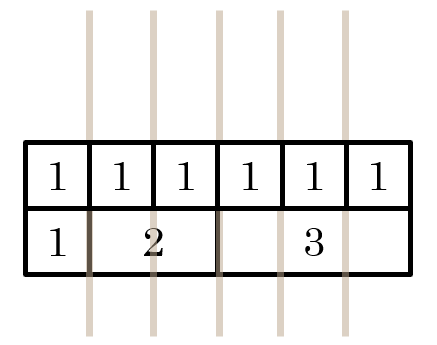
\includegraphics[width=0.5\linewidth]{Bilder/Aufgabe1/Definition_Fugenstellen_Mauer.png}
    \caption{Eine Mauer der Länge 6 besitzt 5 mögliche Fugenstellen.}
\end{figure}

Ähnlich lässt sich auch $f_{Reihe}$ berechnen. Um wissen zu wollen, wie viele freie Fugen eine Reihe mit $n$ Klötzchen besetzen wird, zieht man einfach wieder von der Anzahl der Klötzchen pro Reihe ($n$) 1 ab (siehe Abbildung 6).
\begin{figure}[H]
    \centering
    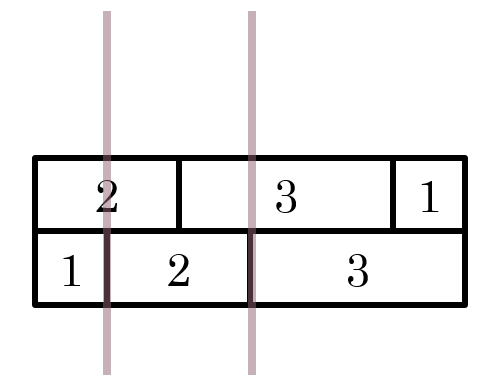
\includegraphics[width=0.5\linewidth]{Bilder/Aufgabe1/Definition_Fugenstellen_Reihe.png}
    \caption{Eine Reihe bei $n = 3$ besetzt $n-1 = 2$ freie Fugen.}
\end{figure}

Daraus ergibt sich die fertige Formel für die Anzahl der Reihen $h$ in einer maximal hohen Mauer in Abhängigkeit von $n$.
\begin{center}
\begin{Large}
\[h = \frac{\frac{n\times(n+1)}{2}-1}{n-1} = \frac{n}{2}+1\]
\end{Large}
\end{center}

%Der Graph der daraus folgenden Funktion
%\begin{center}
%\begin{tikzpicture}
%\begin{axis}[
%xlabel=$n$,
%ylabel=$h$
%]
%\addplot {x/2+1};
%\end{axis}
%\end{tikzpicture}
%\end{center}

% TODO: Ungerades n

%\\[0.4cm]
Die naivste Lösung für die Aufgabe wäre per Brute-Force so lange Klötzchen aneinanderzureihen und Reihen aufeinanderzustapeln, bis man eine fertige Mauer der maximalen Höhe erreicht hat. Jedoch ist die Laufzeit der Brute-Force Methode mit
\begin{center}
\begin{Large}
\[\mathcal{O}(n!^{\lfloor\frac{n}{2}+1\rfloor})\]
\end{Large}
\end{center}
schlechter als exponentiell.
\\[0.4cm]
Für die in der Aufgabenstellung festgelegte Mindestanforderung $n = 10$, gäbe es bereits
\begin{center}
\begin{Large}
\[2.283.380.023.591.730.815.784.976.384.000.000.000.000\]
\end{Large}
\end{center}
\textbf{unterschiedliche Mauerkombinationen} für eine Mauerhöhe von 6.
\\[0.4cm]
Nun ist hierbei allerdings zu beachten, dass es durchaus mehrere mögliche unterschiedliche Lösungen geben kann und das bei der Gesamtmenge unterschiedlicher Mauern auch auf die Reihenfolge von Reihen geachtet wird (siehe Abbildung ||||), welche für die Aufgabenstellung keinen Unterschied macht.
% TODO: Abbildung
\begin{figure}[H]
    \centering
    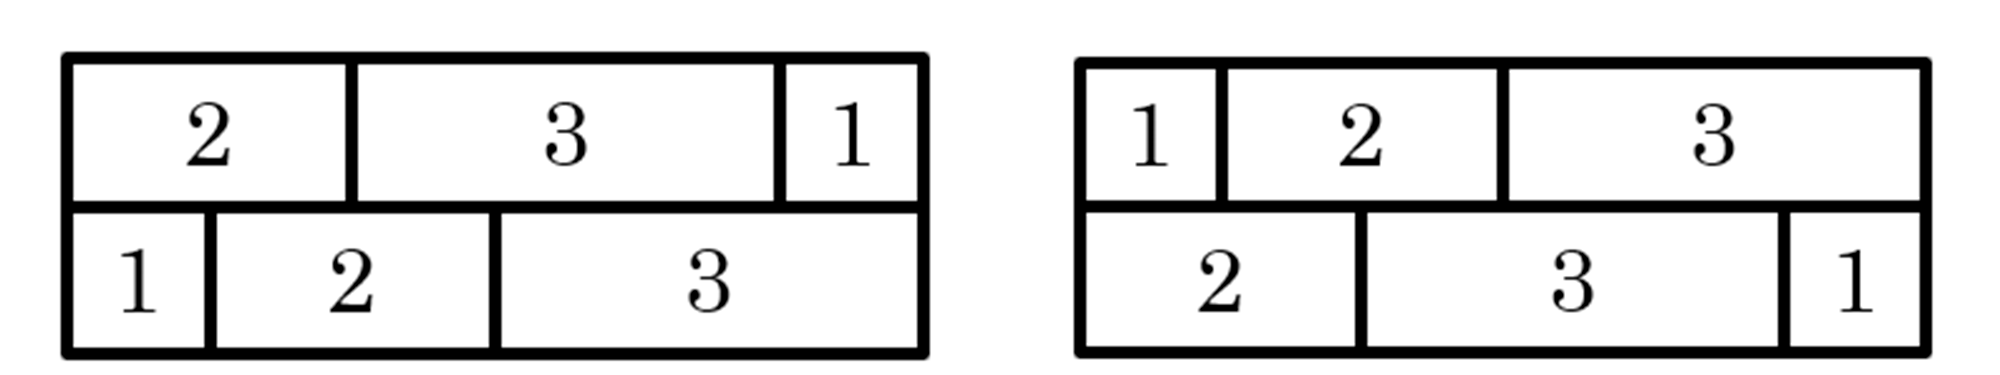
\includegraphics[width=0.9\linewidth]{Bilder/Aufgabe1/Mauervarianten_N3.png}
    \caption{Obwohl beide Mauern aus den selben zwei Reihen bestehen, werden sie als unterschiedliche Mauern angesehen.}
\end{figure}
Weiterhin ist zu beachten, dass es für Mauern mit ungeradem $n$ mehr unterschiedliche Lösungen gibt, als für die wieder darauffolgende Mauer mit geradem $n$.

Dies liegt eben daran, dass bei ungeraden $n$ immer mindestens eine Fugenstelle frei bleibt, was zu mehr richtigen Mauervariationen führt.
\\[0.4cm]
Trotzdem würde das Finden einer Lösung für $n = 10$, selbst wenn ein Computer nur \textbf{1 Millisekunde} für die Permutation einer \textbf{gesamten Mauer} benötigen würde, die maximal erwartete Algorithmuslaufzeit einer BwInf-Lösung bei weitem überschreiten.
\\[0.4cm]
Damit ist eine naive Brute-Force Methode als Lösung ausgeschlossen und es muss nach einem effizienteren Algorithmus gesucht werden.

\subsubsection{Der Algorithmus}
Grundlegend gibt es zwei unterschiedliche Wege eine Mauer, wie in der Aufgabenstellung zu bauen.
\\[0.4cm]
Der offensichtlichere ist die Bauart \textbf{'von unten nach oben'}. Bei dieser Bauart setzt man zuerst die Klötzchen zu einer Reihe zusammen. Hat man eine Reihe fertig, beginnt man mit der zweiten Reihe und so weiter (siehe Abbildung ||||). Man setzt Reihe auf Reihe (von unten nach oben) bis man die Maximalhöhe erreicht hat.
% TODO: Abbildung
\begin{figure}[H]
    \centering
    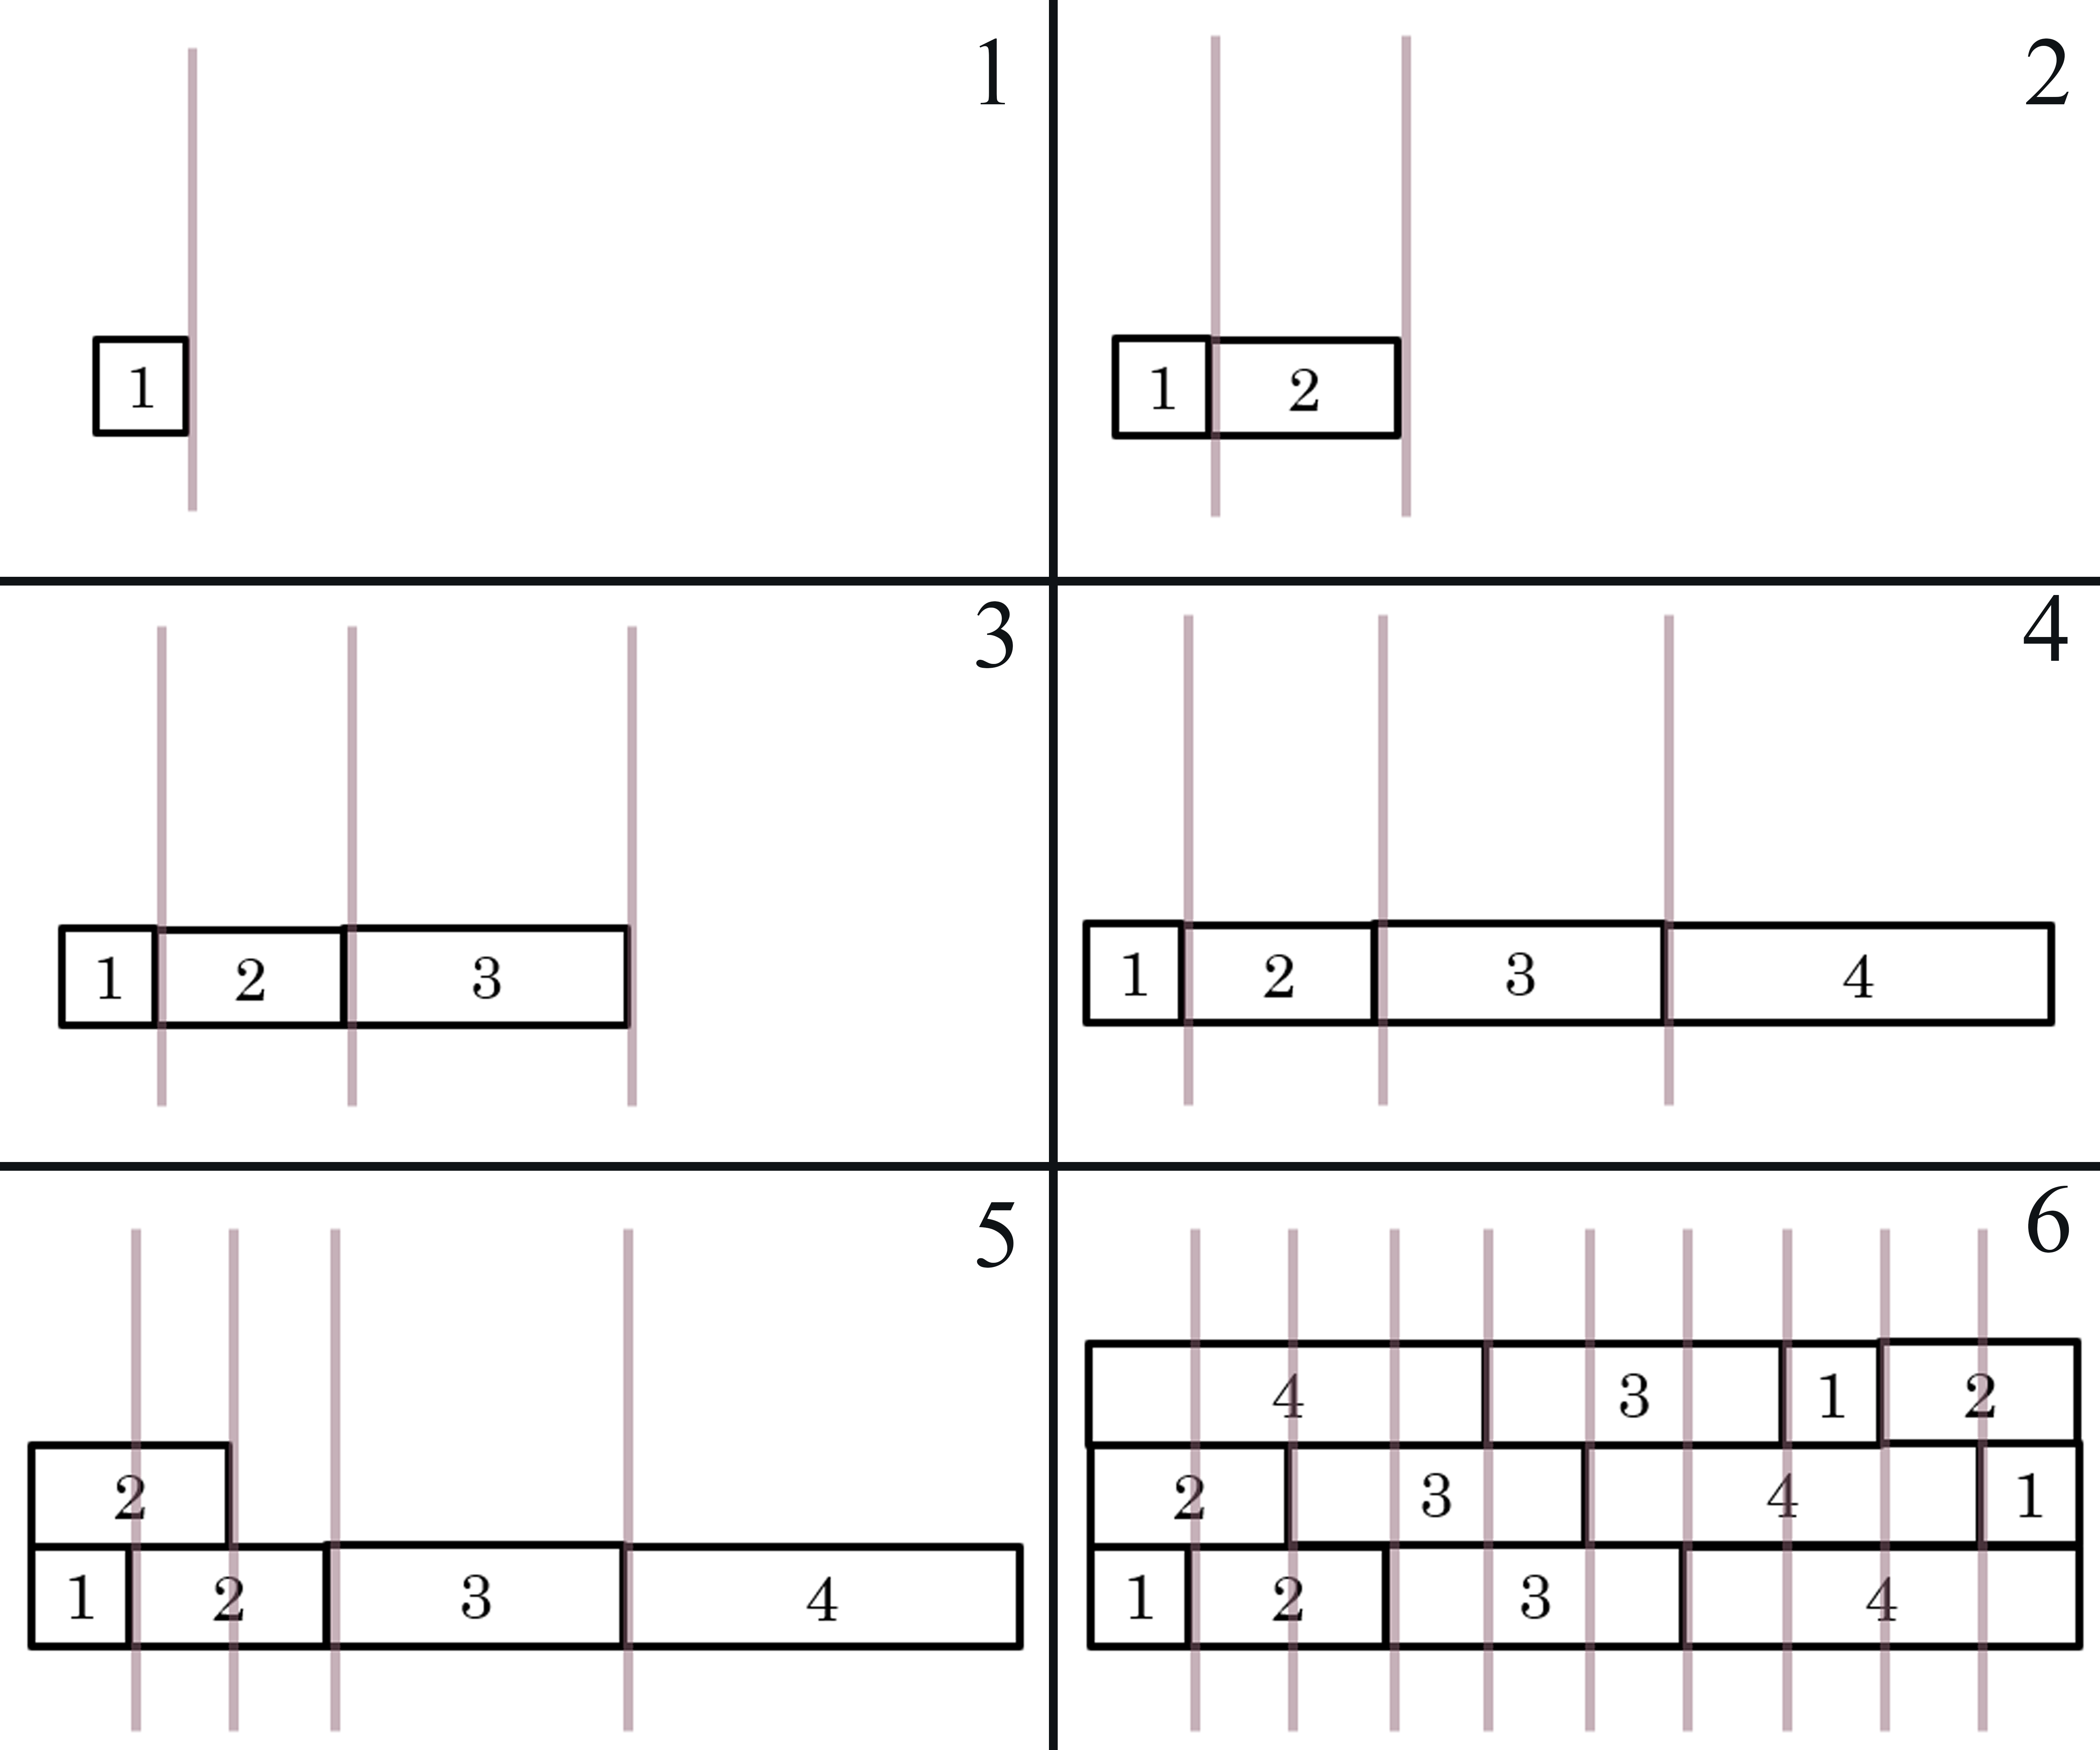
\includegraphics[width=1\linewidth]{Bilder/Aufgabe1/Definition_Mauerbauart_01.png}
    \caption{Der Bau einer Mauer nach der 'von unten nach oben' Methode. Es wird Reihe nach Reihe gebaut, bis die maximale Höhe erreicht wurde.}
\end{figure}

Eine andere Möglichkeit ist, wenn man die Anzahl der Reihen ($h$) für eine Mauer der maximalen Höhe bereits weiß, die Mauer \textbf{'von links nach rechts'} aufzubauen.

\subsection{Implementierung}

\subsection{Laufzeitanalyse}

\subsection{Optimierungsmöglichkeiten}

\subsection{Beispiele}

\subsection{Quellcode}

%===================================================================================
%-------------------------------- AUFGABE 3 ----------------------------------------
%===================================================================================

\newpage
\section{AUFGABE 3 - "Quo vadis, Quax?"}



\subsection{Aufgabenstellung}

\subsection{Lösungsidee}

\subsection{Teilaufgabe (a)}

\subsection{Teilaufgabe (b)}

\subsection{Teilaufgabe (c)}
\subsubsection{Implementierung}
\subsubsection{Laufzeitanalyse}
\subsubsection{Optimierungsmöglichkeiten}
\subsubsection{Beispiele}

\subsection{Teilaufgabe (d)}

\subsection{Quellcode}

%===================================================================================
%---------------------------------- FAZIT ------------------------------------------
%===================================================================================

\newpage
\section{FAZIT}



Lorem ipsum dolor sit amet, consectetur adipiscing elit. Sed tempus consectetur lorem, imperdiet dignissim est auctor a. Vivamus convallis, leo et iaculis egestas, nunc massa porttitor tellus, id faucibus urna justo eget massa. Praesent quis feugiat odio. Nullam quis mattis enim. Fusce volutpat odio in enim sodales venenatis. Mauris consequat.

%===================================================================================
%--------------------------- ABBILDUNGSVERZEICHNIS ---------------------------------
%===================================================================================

\newpage
\section{ABBILDUNGSVERZEICHNIS}
Alle enthaltenen Abbildungen wurden mithilfe von folgenden Tools selbstständig erstellt:
\begin{itemize}
\item Microsoft PowerPoint
\item Grafikrechner - GeoGebra
\item Adobe Photoshop CC 2018 
\end{itemize}

%===================================================================================
%--------------------------- LITERATURVERZEICHNIS ----------------------------------
%===================================================================================

\newpage
\section{LITERATURVERZEICHNIS}

%\begin{thebibliography}{9}
%
%    \bibitem{lamport94}
%      Leslie Lamport,
%      \textit{\LaTeX: a document preparation system},
%      Addison Wesley, Massachusetts,
%      2nd edition,
%      1994.
%    
%\end{thebibliography}

%===================================================================================
%------------------------- ERKLÄRUNG DES VERFASSERS --------------------------------
%===================================================================================

\newpage
\section{ERKLÄRUNG DES VERFASSERS}



Lorem ipsum dolor sit amet, consectetur adipiscing elit. Sed tempus consectetur lorem, imperdiet dignissim est auctor a. Vivamus convallis, leo et iaculis egestas, nunc massa porttitor tellus, id faucibus urna justo eget massa. Praesent quis feugiat odio. Nullam quis mattis enim. Fusce volutpat odio in enim sodales venenatis. Mauris consequat.

\begin{figure}[H]
    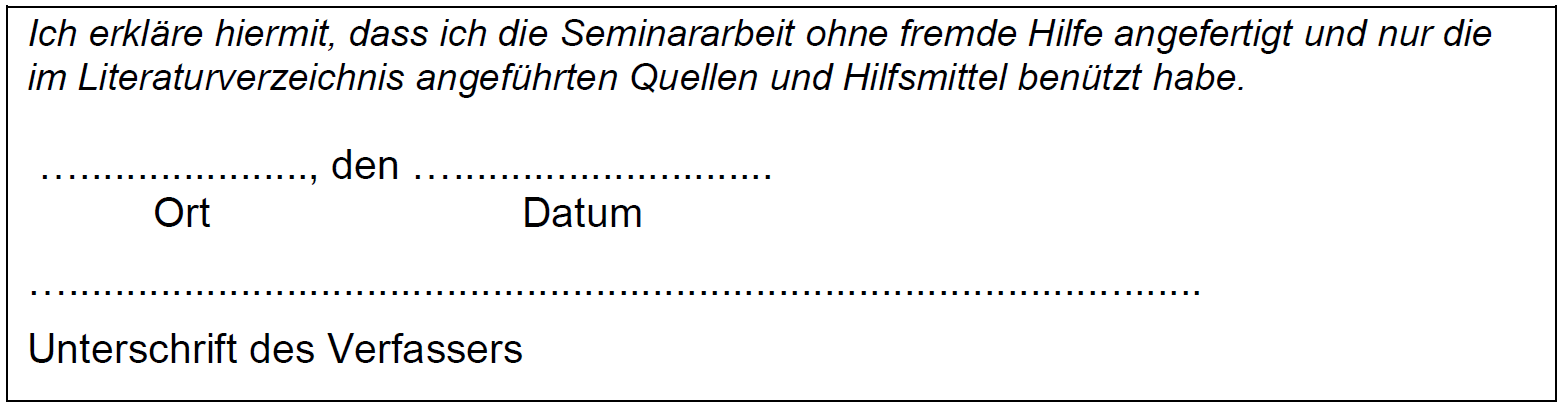
\includegraphics[width=\linewidth]{Bilder/Sonstiges/ErklaerungDesVerfassers.png}
\end{figure}

\end{document}